\documentclass[a4paper,12pt]{article}
\usepackage[margin=1in,left=1in,includefoot]{geometry}
\usepackage[margin=1in,left=1in,includefoot]{geometry}
\usepackage{multicol}
\setlength{\columnsep}{-12cm}
\usepackage[tbtags]{amsmath}%%%%%
%%%%%%%%%%%%%%%%%%%%%%%%%
 \usepackage{amsmath}
 \usepackage{amsfonts}
 \usepackage{amssymb}
\usepackage{mathtools}
\usepackage{amsthm}
\everymath{\displaystyle}
\usepackage[T1]{fontenc}
\usepackage{mathpazo}%%palatino font for text
\usepackage[euler-digits,euler-hat-accent]{eulervm}%euler for math font
%%%%%%%%%%%%%%%%%%%%%%%%%%%%%%%%%%%%
%%%%%%%%%%%%%%%%%%%%%%%%%%%%%%%%%%%%
\usepackage{ragged2e}%%%%%%%%%%%%%%for \justify
%%%%%%%%%%%%%%%%%%%%%%%%%%%%
\usepackage[dvipsnames]{xcolor}
\usepackage{xcolor}
\usepackage{booktabs,tabularx}
\usepackage{multirow}
\usepackage{tikz}
\usepackage{graphicx} % Required for including images
\usepackage[font=small,labelfont=bf]{caption} % Required for specifying captions to tables and figures
%%%%%%%%%%%%%%%%%%%%%%%%%%%%%%%%
\usepackage[colorlinks=true]{hyperref}%
 %%%%%%%%%%%%%%%%%%%%%%%%%%%%%%%%%%%%%
\usepackage{fontspec}
\usepackage[ethiop,main=english]{babel}
\newfontface{\geezfont}{FreeSerif}
\newenvironment{geez}{\geezfont}{}
\lccode`፡=`፡  \catcode`፡=11
\lccode`።=`። \catcode`።=11
\babelprovide[import,
  onchar = fonts ids,
  typography/intraspace = 0 .1 0,
  typography/linebreaking = s, 
  characters/ranges = 1200..139F 2D80..2DDF AB00..AB2F,
  ]{amharic}
\babelfont[amharic]{rm}{FreeSerif}
%%%%%%%%%%%%%%%%%%%%%%%%%%%%%%%%%%%%%%%%%%%%%%%%
%%%%%%%%%%%%%%%%%%%%%%%%%%%%%%%%%%%%%%%%%%%%%%%%%%%%
\newtheoremstyle{mystyle}%                % Name
  {}%                                     % Space above
  {}%                                     % Space below
  {\itshape}%                             % Body font
  {}%                                     % Indent amount
  {\bfseries}%                            % Theorem head font
  {.}%                                    % Punctuation after theorem head
  { }%                                    % Space after theorem head, ' ', or \newline
  {}%                                     % Theorem head spec (can be left empty, meaning `normal')
%%%%%%%%%%%%%%%%%%%%%%%%%%%%%%%%%%%%%%%%%%%%%%%%%%%%%%%%%%%%%%%%%%%%%
\theoremstyle{mystyle}
\newtheorem{theorem}{Theorem}
\newtheorem{proposition}{Proposition}
\newtheorem{lemma}{Lemma}
\newtheorem{corollary}{Corollary}
\newtheorem{example}{Example}
\newtheorem{solution}{Solution}
\newtheorem{conclusion}{Conclusion}
\newtheorem{definition}{Definition}
\newtheorem{remark}{Remark}
\newtheorem{amharicdefinition}{\begin{geez}ትርጉም\end{geez}}
%%%%%%%%%%%%%%%%%%%%%%%%%%%%%%%
%%%%%%%%%%%%%%%%%%%%%%%%%%%%%%%%%%%%%%%%%%%%%%%%%
\numberwithin{equation}{section}
\numberwithin{theorem}{section}
\numberwithin{proposition}{section}
\numberwithin{example}{section}
\numberwithin{remark}{section}
\numberwithin{lemma}{section}
\numberwithin{corollary}{section}
\numberwithin{definition}{section}
\numberwithin{amharicdefinition}{section}
%%%%%%%%%%%%%%%%%%%%%%%%%%%%%%%%%%%%%%%%%%%%%%%%%%
%%%%%%%%%%%%%%%%%%%%%%%%%%
\usepackage[shortlabels]{enumitem}
\usepackage{soul}%%for highlighting texts and equations begin inside $$..\hl{some text here}
\newcommand{\mathcolorbox}[2]{\colorbox{#1}{$\displaystyle #2$}}%%to highlight math equations which is inside \begin{equation}...\end{equation}
\usepackage{authblk}
\title{ {\small Received: March 22, 2024\\ Accepted: January 16, 2025\\ Published: March 4, 2025}\\[2cm]
{\large General Knowledge 0.3 For Pin Number 6}
}
\author[1,2,$*$]{\small Dagnachew Jenber}
%\author[2]{second author}
%\author[3]{third author}
%\author[4]{fourth author}
\affil[1]{ Department of Mathematics, Bahir Dar University, Bahir Dar, Ethiopia.}
\affil[2]{Department of Mathematics, Addis Ababa Science and Technology University, Addis Ababa, Ethiopia.}
%\affil[3]{third affilation}
%\affil[4]{fourth affilation}
\affil[$*$]{Corresponding author: Dagnachew Jenber, dagnachew.Jenber@aastu.edu.et}
\setcounter{Maxaffil}{0}
\renewcommand\Affilfont{\itshape\small}
\usepackage{xhfill}
\setlength{\parindent}{0pt}
%%%%%%%%%%%%%%%%%%%%%%%%%%%%%%%%%%%%%%%%%%%%%
%%%%%%%%%%%%%%%%%%%%%%%%%%%%%%%%%%%%%%%%%%%%%%%%%%%%%%%%%%
\usepackage[backend=bibtex,maxnames=1000,minnames=10,maxalphanames=1000,
minalphanames=10,style=numeric,sorting=anyt,firstinits=true]{biblatex}
\DeclareNameAlias{default}{last-first}
\addbibresource{gk0.3p6.bib}
\renewbibmacro{in:}{}
%%%%%%%%%%%%%%%%%%%%%%%%%%%%%
\usepackage[tbtags]{amsmath}%%%%%https://tex.stackexchange.com/questions/368353/using-equation-split-how-can-i-ensure-that-only-the-last-equation-is-numbered%%%%
%%%%%%%%%%%%%%%%%%%%%%%%%
\usepackage{geometry}
\usepackage{graphicx}
\makeatletter         
\def\@maketitle{
\raggedright
\begin{multicols}{2}
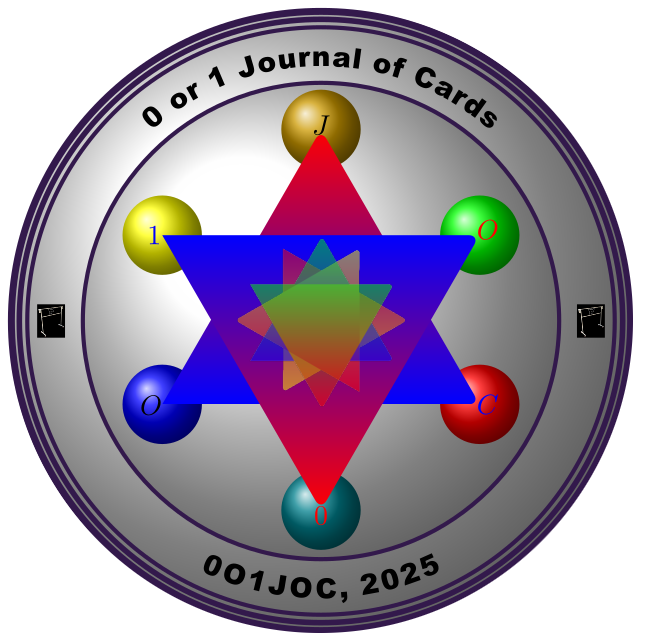
\includegraphics[width = 1.8cm]{0O1JOC}
\vfill\null\columnbreak
0 or 1 Journal of Cards for General Knowledge 0\\
Volume-1(2025), Issue-1, 4 pages
\end{multicols}
\begin{center}
{\large \bfseries \sffamily \@title }\\[1.5ex]
{  \@author}\\[8ex]
\end{center}}
\makeatother
%%%%%%%%%%%%%%%%%%%%%%%%%%%%%%%%%%%%%%%%%%%%%%%
\makeatletter
\renewcommand\tableofcontents{%
  \null\hfill\textbf{\Large\contentsname}\hfill\null\par
  \@mkboth{\MakeUppercase\contentsname}{\MakeUppercase\contentsname}%
  \@starttoc{toc}%
}
\makeatother
%%%%%%%%%%%%%%%%%%%%%%%%%%%%%%%%%%%%%%%%%%%%%%%%%%%
%%%%%%%%%%%%%%%%%%%%%%%%%%%%%%%%%%%%%%%%%%%%%%%%%%%%%
\usepackage{hyperref}% http://ctan.org/pkg/hyperref
%%%%%%%%%%%%%%%%%%%%%%%%%%%%%%%%%%%%

%%%%%%%%%%%%%%%%%%%%%%%%%%%%%%%%%%%%%%
%%%%%%%%%%%%%%%%%%%%%%%%%%%%%%%%%%%%%%%%
\begin{document}
\maketitle
\fontfamily{kpfonts}
\hypersetup{
  colorlinks,
  citecolor=red,
  linkcolor=red,
  urlcolor=blue}

  \hypersetup{
  citebordercolor=red,
  filebordercolor=red,
  linkbordercolor=blue
}
\centering
{\bf Abstract}
\justify
This work presents 30 number of cards from different discplines focused on english, physics and mathematics subject. The jester cards are extraneous, Provocative, acceleration, Rational Number, Integer Number and Rakish.
\renewcommand{\thefootnote}{}%remove numbering for the footnote
\footnotetext{\scriptsize \textcopyright\ The Author(s) 2025. Open Access This article is licensed under a Creative Commons Attribution-NonCommercial-NoDerivatives
4.0 International License, which permits any non-commercial use, sharing, distribution and reproduction in any medium or format, as long as you give appropriate credit to the original author(s) and the source, provide a link to the Creative Commons licence, and indicate if you modified the licensed material. You do not have permission under this licence to share adapted material derived
from this article or parts of it. The images or other third party material in this article are included in the article’s Creative Commons licence, unless indicated otherwise in a credit line to the material. If material is not included in the article’s Creative Commons licence and your intended use is not permitted by statutory regulation or exceeds the permitted use, you will need to obtain
permission directly from the copyright holder. To view a copy of this licence, visit \url{https://creativecommons.org/licenses/by-nc-nd/4.0/}.}
\renewcommand{\thefootnote}{\arabic{footnote}}%%restore default numbering for future footnotes
\section{\begin{geez}መግቢያ\end{geez}}
\label{S:2}
አሁን ባለንበት ዘመን የአንባቢያን ማህበረሰብ እየቀነሰ መምጣት አሳሳቢ ደረጃ ላይ ደርሷል። በብዙ ምክኒያት ሰወች ቁጭ ብለው
ማንበብ የተውበት ጊዜ ነው። ለምሳሌ ጠቃሚ ያልሆነ ሶሻል
ሚዲያ ላይና በአልባሌ ቦታወች ጊዜን ማጥፋት ከብዙወቹ ትንሾቹ ምክኒያቶች ናቸው። በ2017 ዓ.ም ዳኛቸው ለዚህ የሚሆን መፍትሄ ብሎ ያቀረበው 0 ወይም 1 ጨዋታ በሚል ርእስ የተዘጋጀ ትልቅ አክሲዮን ማህበር አለ። ይህ አክሲዮን ማህበር ከላይ የተጠቀሰውን ችግር በሚከተሉት መልኩ መፍታት ይቻላል ብሎ ያምናል። በዚህ ፅሁፍ ውስጥ የተካተተው መፍትሄ አሳማኝ ሆኖ አግኝተነዋል (ለበለጠ መረጃ የ 0 ወይም 1 መመስረቻ ፅሁፍን ይመልከቱ)። በዚህ አክሲዮን ማህበር የቀረበውን መፍትሄ ባጭሩ እንደሚከተለው አስቀምጠነዋል። 
\begin{enumerate}
\item[(1)] ማንበብን ወይም ጥናትን መዝናኛና ገንዘብ ማግኛ እንዲሁም ደግሞ ሽልማት የሚያስገኝ ማድረግ። ከማጥኛ ወይም አዲስ እውቀትን ከማግኛ  ዘዴወች ውስጥ አንደኛው ነገሮችን በተመሳሳያቸው በማዛመድ ማወቅ ነው። ለምሳሌ የአንድ እንግሊዘኛ ቃል ብዙ ተመሳሳይ ቃላቶች አሉት። እነሱን በማዛመድ ለመሸምደድ መሞከር ጥሩ ከሚባሉት ዘዴወች ውስጥ አንዱ ነው። ግን ደግሞ ይሄን ልምምዶሽ አይረሴ ለማድረግ በጨዋታ መልክ ሆኖ በቡድን እየተዝናኑና እየተወያዩ ሲሆን ተመራጭ ያደርገዋል።
ካርድ በማዘጋጀት የእንግሊዘኛ ቃላቶችን ማጥናት በሚል ዙሪያ የተጠኑ ሳይንሳዊ ጥናቶች አሉ (ለምሳሌ፣ እነዚህን ይመልከቱ፣ 
\cite{aslan2011teaching,azabdaftari2012comparing,bryson2012using,kosim2013improving,
 nikoopour2014vocabulary,
nugroho2012improving,
saputri2017improving,senzaki2017reinventing,sitompul2013teaching,
wahyuni2014flashcards})
\item[(2)] ነገሮችን በአይነት አይነታቸው እያዛማዱ ማወቅ ያመራምራል፣ ጠያቂ ያደርጋል፣ ከጓደኛ ጋር ያከራክራል፣ ማመሳከሪያ መፅሃፍ ፍለጋ እስከመሄድ ድረስ ያደርሳል። እናም በዚህ መልክ ሲሆን ያን ነገር ለመርሳት ብዙ ጊዜ ይጨርሳል። 
\item[(3)] ማዛመድን ደግሞ ከጓደኛ ጋር ሆነው እየተዝናኑ በጨዋታ መልክ ካደረጉትና እውቀትንና ማወቅን ለማበረታት ደግሞ ለአሸናፊው ጉርሻ በመስጠት ከሆነ ጨዋታውም ተወዳጅ ይሆናል ማለት ነው።
\item[(4)] ከላይ ከ1-3 የተጠቀሱትን መፍትሔወች ለማከናወን የተለያዩ አይነት አዝናኝ ጨዋታወችን ማዘጋጀት።
\end{enumerate}
በዚህ ወረቀት ውስጥ፣ ለ 0 ወይም 1 ጨዋታ የሚሆን ካርድን አዘጋጅተናል። ያዘጋጀነው ካርድ ለጠቅላላ እውቀት 0.3 የሚሆን ሲሆን ከዚህ በፊት ያልተዘጋጁ ካርዶችን የሚዳስስ ነው። ያዘጋጀነውን የካርዶቹን መረጃ ባጭሩ እንደሚከተለው ገልፀነዋል። የመርፌ ብዛት=6 እና k=3 ቢሆኑ። ስለዚህ n=8*3+6=30 ይሆናል። ስለዚህ አጫዋች ካርዶችን ጨምሮ ባጠቃላይ 30 ካርዶች አሉ። ተጫዋች ካርዶች፤ $30-6=24$ ካርዶች ይሆናሉ፤ 24 ደግሞ የ 8 ብዜት ነው (ለበለጠ መረጃ የዜሮ ወይም አንድ መመስረቻ ፅሁፍን ይመልከቱ)።  አጫዋች ካርዶች የሚከተሉት ናቸው፤ extraneous፣ Provocative፣ Rakish፣ Acceleration፣ Rational number እና  Integer number ናቸው።
\section{\begin{geez}አጫዋች ካርዶች (Jester Cards)\end{geez}}
\label{S:2}
\begin{definition}[Extraneous]Something that is not essential or relevant to the matter at hand. (see, \cite{dictionary2002merriam}).\\
Example: In solving the equation , the solutions are valid, but if we square both sides of an equation like and get , the solution would be extraneous.
\end{definition}
\begin{definition}[Provocative]Causing a strong reaction, often in a deliberate way; intended to stimulate thought, debate, or controversy.  (see,  \cite{dictionary1989oxford}).\\
Example: A provocative article questioning the validity of established scientific theories may spark debate in the academic community.
\end{definition}
\begin{definition}[Rakish] Rakish describes someone who is stylishly unconventional or morally questionable, often with a carefree or dashing appearance. (see, \cite{dictionary2002merriam}).\\
Example: He had a rakish charm, with his unbuttoned shirt and confident smirk, making him seem both attractive and rebellious.
\end{definition}
\begin{definition}[Acceleration] Acceleration is the rate of change of velocity of an object with respect to time. Mathematically, it is given by:
$a = \frac{dv}{dt}$  (see, \cite{serway2018current}).\\
Example: A car increasing its speed from 20 $m/s$ to 30 $m/s$ in 5 seconds has an acceleration of: $a = \frac{30 - 20}{5} = 2 \text{ m/s}^2$.
\end{definition}
\begin{definition}[Rational Number] A rational number is any number that can be expressed as the quotient or fraction $\frac{p}{q}$ , where $p$ and $q$ are integers, and $q\ne 0$. The set of rational numbers is denoted by $\mathbb{Q}$. For more see \cite{stewart2012calculus}.\\
Example: The numbers $\frac{3}{4}$, $-2$(which can be written as $\frac{-2}{1}$ ), and 0.75 (which is  $\frac{3}{4}$) are rational numbers.
\end{definition}
\begin{definition}[Integer number] An integer is any whole number, including positive numbers, negative numbers, and zero, denoted by:
$\mathbb{Z} = \{ \dots, -3, -2, -1, 0, 1, 2, 3, \dots \}$  (see, \cite{stewart2012calculus}).\\
Example: -5, 0, and 12 are all integers
\end{definition}
\section{\begin{geez}ተጫዋች ካርዶች ከነአጫዋቻቸው (Player Cards with their Jester)\end{geez}}
\label{S:3}
\begin{enumerate}
\item extraneous=external=outside=exterior=outward=alien=foreign=extrinsic.
\item provocative=suggestive=erotic=indecent=titillating.
\item Rakish=dashing=sporty=stylish=debonair=jaunty=dapper=disreputable.
\item acceleration=(change in velocity)/(change in time)=rate at which velocity changes with time, in terms of both speed and direction.
\item $\mathbb{Q}$=mathematical symbol for the set of rational numbers=$\{\frac{a}{b}, ~b\ne 0\}$, where $a$ and $b$ are integers.
\item $\mathbb{Z}$=mathematical symbol for the set of integers=$\{\cdots,-3,-2,-1,0, 1,2,3,\cdots\}$.
\end{enumerate}
\printbibliography
\end{document}
